\thispagestyle{toancuabinone}
\pagestyle{toancuabi}
\everymath{\color{toancuabi}}
%\blfootnote{$^1$\color{toancuabi}Đại học Thăng Long.}
\graphicspath{{../toancuabi/pic/}}
\begingroup
\AddToShipoutPicture*{\put(0,616){\includegraphics[width=19.3cm]{../bannertoancuabi}}}  
\AddToShipoutPicture*{\put(40,550){\includegraphics[scale=1]{../tieude1.pdf}}} 
\centering
\endgroup
\vspace*{155pt}

\begin{multicols}{2}
	Tính diện tích của một hình là một chủ đề hay và có nhiều điều thú vị của các bạn nhỏ cuối cấp $1$. Chủ đề này cũng được các thầy cô trong Câu lạc bộ Unicorn Math Circle (UMC) giảng dạy trong nhiều buổi với sự tham gia hào hứng của các bạn học và có nhiều cách giải độc đáo đã được đưa ra. Chúng ta cùng bắt đầu với một dạng tính diện tích trong những bài giảng của các thầy cô -- Tính diện tích hình trên lưới ô vuông. Với cách tính được trình bày trong bài viết này, các bạn nhỏ chưa học đến những công thức tính diện tích vẫn có thể tính được diện tích của nhiều kiểu hình khác nhau nhé, vì chúng ta chỉ dựa vào các ô vuông trên lưới thôi. Hơn thế nữa, dựa vào lưới ô vuông các em còn được khám phá những định lý nổi tiếng như Định lý Pythagoras, Định lý Pick và những tính chất hay khác của Toán học.
	\vskip 0.1cm
	$\pmb{1.}$ \textbf{\color{toancuabi}Diện tích của những hình cơ bản}
	\begin{figure}[H]
			\centering
			\vspace*{-5pt}
			\captionsetup{labelformat= empty, justification=centering}
			\includegraphics[width=0.45\linewidth]{1}
			\caption{\small\textit{\color{toancuabi}Hình $1$.}}
			\vspace*{-10pt}
		\end{figure}
	Như nhiều bạn đã biết, lưới ô vuông gồm các đường thẳng song song cách đều nhau theo cả chiều ngang cũng như chiều dọc và tạo thành những hình vuông mà ta quy ước là chiếm $1$ đơn vị diện tích. Hình vuông đơn vị này là cơ sở để chúng ta tính diện tích của các hình tạo ra trên lưới trong các phần dưới đây.
	\vskip 0.1cm
	Trước hết ta bắt đầu với việc tìm diện tích của những hình rất đơn giản nhưng đóng vai trò quan trọng trong việc tính toán diện tích các hình ở các ví dụ sau.
	\vskip 0.1cm
	Hình cơ bản đầu tiên cần tính diện tích là hình vuông và hình chữ nhật có các cạnh nằm trên các đường thẳng của lưới.
	\vskip 0.1cm
	\textbf{\color{toancuabi}Ví dụ} $\pmb{1.}$ Tính diện tích của hai hình được tô đậm trong lưới ô vuông dưới đây.  
	\begin{figure}[H]
		\centering
		\vspace*{-10pt}
		\captionsetup{labelformat= empty, justification=centering}
		\includegraphics[width=0.4\linewidth]{2}
		\includegraphics[width=0.45\linewidth]{3}
		\caption{\small\textit{\color{toancuabi}Hình $2$ \hspace*{40pt}Hình $3$.}}
		\vspace*{-15pt}
	\end{figure}
	\textit{Lời giải.} Bằng cách đếm trực tiếp, ta thấy
	\vskip 0.1cm
	-- Hình $A$ có tổng cộng $9$ ô vuông nên có diện tích là $9$ đơn vị;
	\vskip 0.1cm
	-- Hình $B$ có tổng cộng $12$ ô vuông nên có diện tích phần hình bằng $12$ đơn vị.
	\vskip 0.1cm
	Các bạn mà học công thức tính diện tích hình vuông và hình chữ nhật rồi thì có thể nhận thấy ngay kết quả trên có thể tính được bằng cách sau.
	\vskip 0.1cm
	-- Cạnh của hình vuông là $3$ đơn vị nên diện tích là: $3 \times  3 = 9$ đơn vị;
	\vskip 0.1cm
	-- Hình chữ nhật chiều dài và chiều rộng tương ứng là $4$ và $3$ đơn vị nên có diện tích là: $4 \times  3 = 12$ đơn vị.
	\vskip 0.1cm
	Chúng ta tiếp tục với một hình cơ bản nữa là tam giác có hai cạnh trùng với hai đường dọc và ngang của lưới ô vuông.
	\vskip 0.1cm
	\textbf{\color{toancuabi}Ví dụ} $\pmb{2.}$ Tính diện tích tam giác được tô đậm trong hình dưới đây.
	\begin{figure}[H]
		\centering
		\vspace*{-5pt}
		\captionsetup{labelformat= empty, justification=centering}
		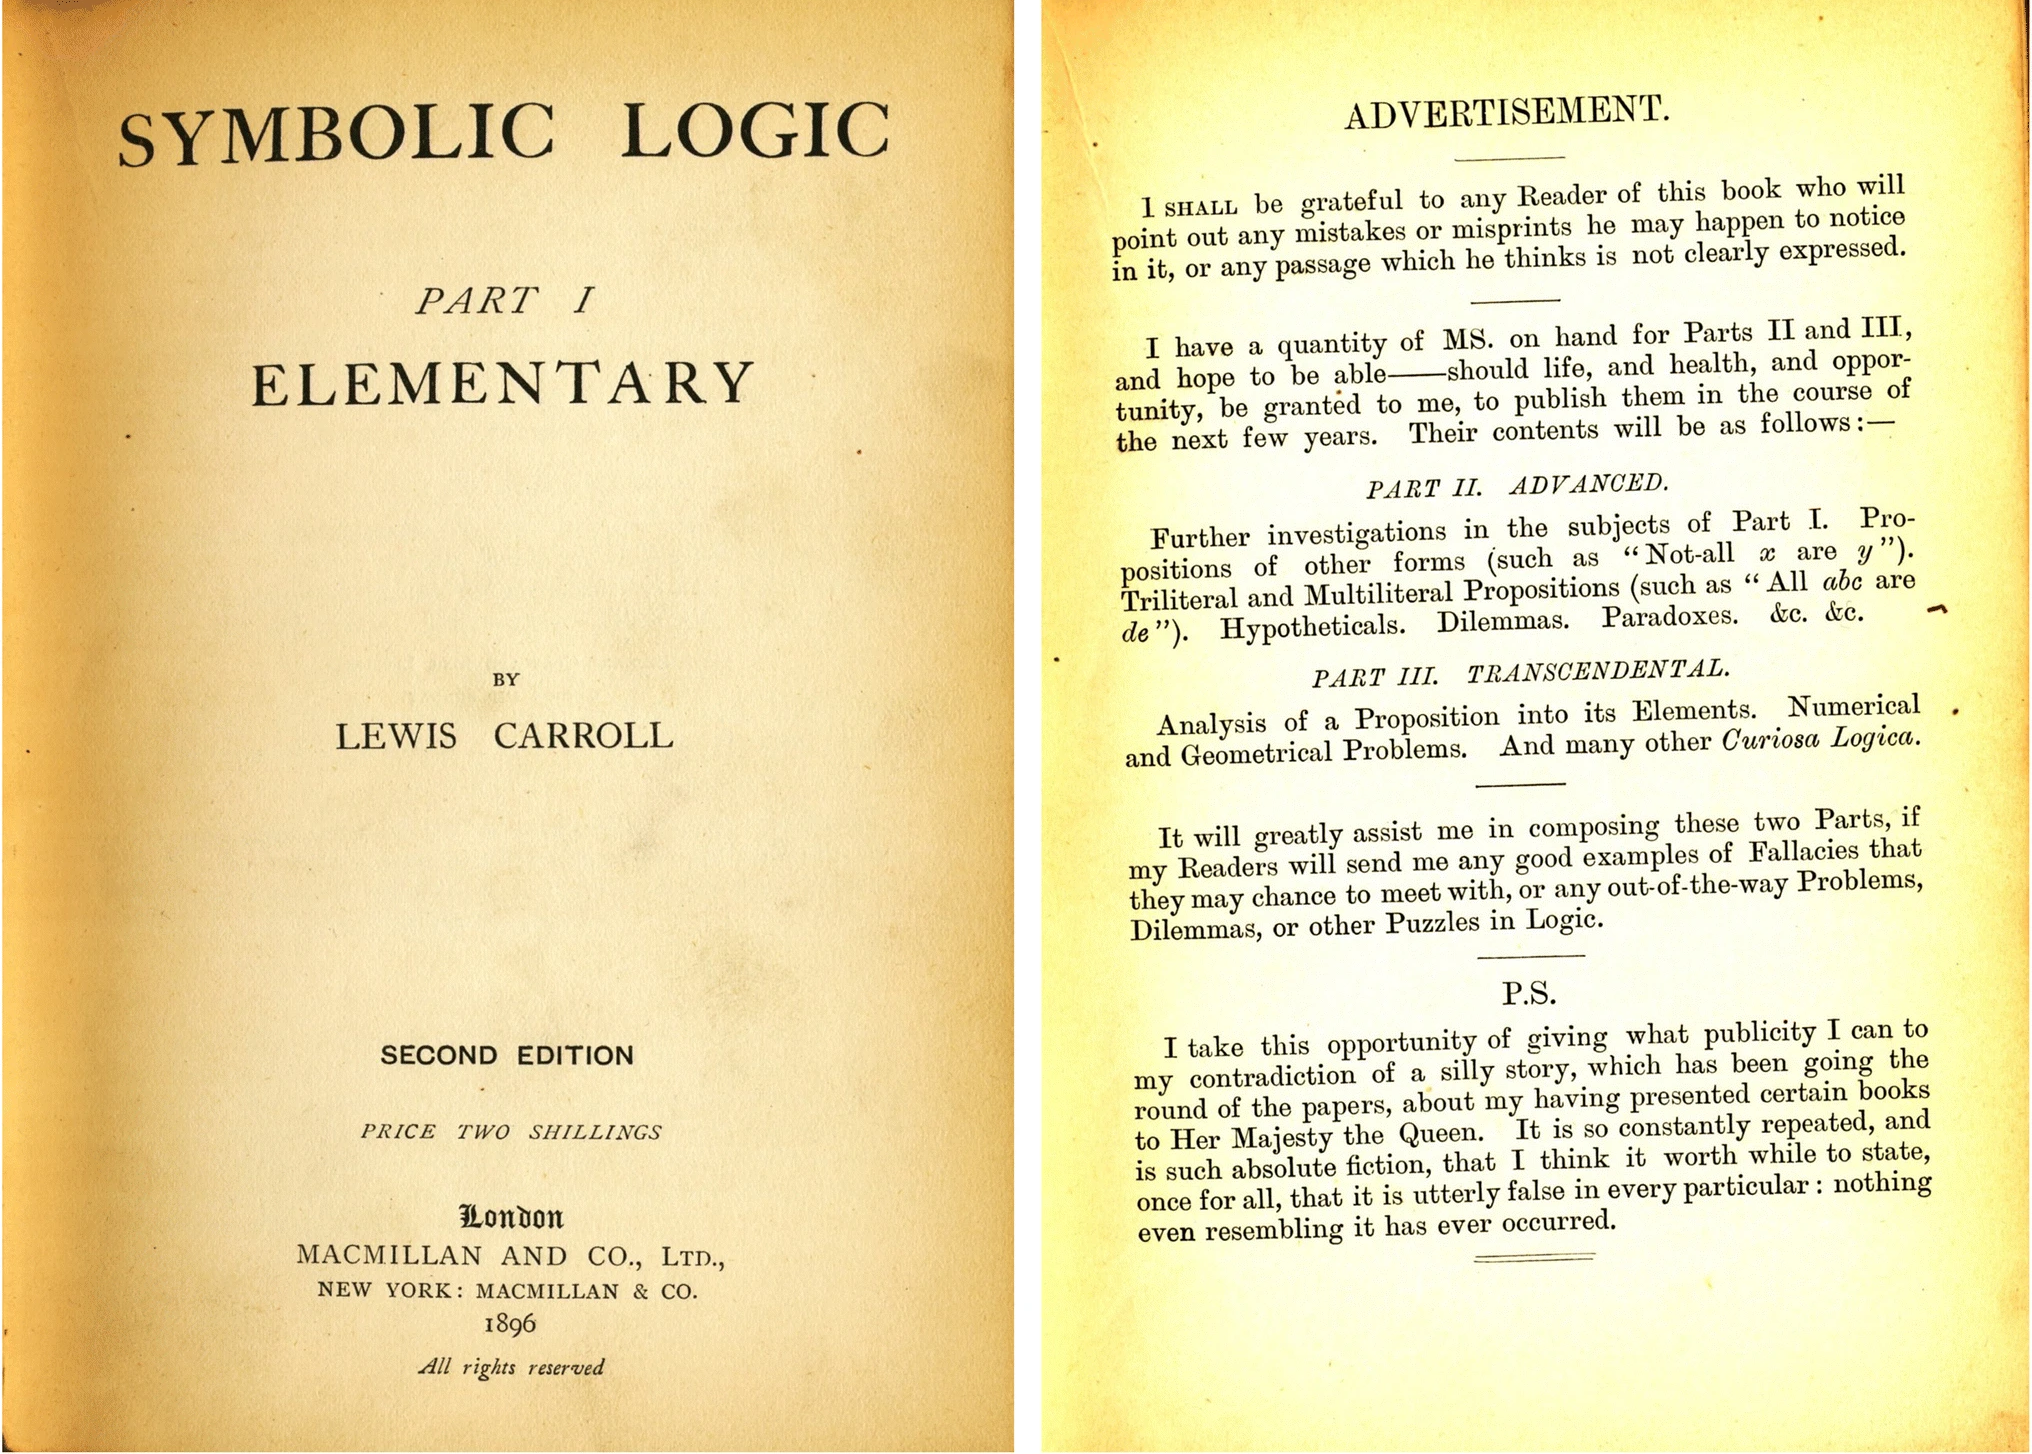
\includegraphics[width=0.5\linewidth]{4}
		\caption{\small\textit{\color{toancuabi}Hình $4$.}}
		\vspace*{-15pt}
	\end{figure}
	\textit{Lời giải.} Ở ví dụ này, các bạn nhỏ quan sát một chút thì sẽ thấy ngay diện tích của tam giác đã cho bằng một nửa hình chữ nhật màu cỡ $6\times 4$ được tô màu xanh dương dưới đây.
	\begin{figure}[H]
		\centering
		\vspace*{-5pt}
		\captionsetup{labelformat= empty, justification=centering}
		\includegraphics[width=0.5\linewidth]{5}
		\caption{\small\textit{\color{toancuabi}Hình $5$.}}
		\vspace*{-15pt}
	\end{figure}
	Do diện tích hình chữ nhật được tạo bởi $24$ ô vuông nên diện tích hình tam giác bằng $\dfrac{24}{2}=12$ (đơn vị diện tích).
	\vskip 0.1cm
	Ngoài ra, nếu bạn nhỏ nào đã biết công thức tính diện tích tam giác thì hình trong Ví dụ $2$ là tam giác vuông với $2$ cạnh góc vuông là $6$ và $4$ đơn vị. Do đó diện tích của tam giác là $\dfrac{1}{2}\times 6\times 4 = 12$ đơn vị.
	\vskip 0.1cm
	Hai ví dụ trên cho ta một cái nhìn trực quan về bài toán tính diện tích trên lưới ô vuông, ta chỉ đơn giản dùng cách đếm đơn thuần số ô vuông trên lưới. Trong các bài toán sau, có thể có nhiều cách giải khác nhau nhưng bài viết đưa ra cách giải mà chỉ dựa vào những hình cơ bản đã biết cách tính diện tích trong Ví dụ $1$ và Ví dụ $2$.
	\vskip 0.1cm
	$\pmb{2.}$ \textbf{\color{toancuabi}Diện tích hình chia thành những hình cơ bản}
	\vskip 0.1cm
	Chúng ta lại tiếp tục với tính diện tích của tam giác nhé. Lần này là tam giác chỉ có một cạnh trùng với đường dọc--ngang của lưới và nhận thấy ta không thể áp dụng luôn cách tính như trong Ví dụ $2$. Tuy nhiên bằng cách chia tam giác đã cho thành các tam giác nhỏ có hai cạnh trùng với những đường thẳng của lưới, ta hoàn toàn có thể áp dụng cách tính diện tích tam giác như trong tình huống trên.
	\vskip 0.1cm
	\textbf{\color{toancuabi}Ví dụ} $\pmb{3.}$ Tính diện tích tam giác được tô đậm trong hình cho ở dưới đây.
	\begin{figure}[H]
		\centering
		\vspace*{-5pt}
		\captionsetup{labelformat= empty, justification=centering}
		\includegraphics[width=0.5\linewidth]{6}
		\caption{\small\textit{\color{toancuabi}Hình $6$.}}
		\vspace*{-10pt}
	\end{figure}
	\textit{Lời giải.} Ta chia hình tam giác lớn thành hai hình tam giác $(1)$ và $(2)$.
	\begin{figure}[H]
		\centering
		\vspace*{-5pt}
		\captionsetup{labelformat= empty, justification=centering}
		\includegraphics[width=0.5\linewidth]{7}
		\caption{\small\textit{\color{toancuabi}Hình $7$.}}
		\vspace*{-10pt}
	\end{figure}
	Sau đó tính diện tích từng tam giác, tương tự như trong Ví dụ $2$.
	\begin{figure}[H]
		\centering
		\vspace*{-5pt}
		\captionsetup{labelformat= empty, justification=centering}
		\includegraphics[width=0.5\linewidth]{8}
		\caption{\small\textit{\color{toancuabi}Hình $8$.}}
		\vspace*{-5pt}
	\end{figure}
	Hình tam giác $(1)$ có diện tích bằng một nửa hình chữ nhật bên trái nên có diện tích là: $\dfrac{10}{2}=5$ (đơn vị diện tích).
	\vskip 0.1cm
	Hình tam giác $(2)$ có diện tích bằng một nửa hình chữ nhật bên phải và do đó có diện tích là: $\dfrac{20}{2}=10$ (đơn vị diện tích).
	\vskip 0.1cm
	Suy ra hình cần tính có diện tích bằng $5+10=15$ (đơn vị diện tích). 
	\vskip 0.1cm
	Tính diện tích bằng cách chia hình thành những hình nhỏ hơn không chỉ dừng lại ở việc tính toán những dạng hình học quen thuộc như hình tam giác, hình chữ nhật, ... mà còn có thể áp dụng cho rất kiểu hình khác nhau. Chẳng hạn như hình ``chú mèo`` ngộ nghĩnh dưới đây.  
	\vskip 0.1cm
	\textbf{\color{toancuabi}Ví dụ} $\pmb{4.}$ Tính diện tích ``chú mèo`` được cho bởi phần tô đậm trong hình sau.
	\begin{figure}[H]
		\centering
		\vspace*{-5pt}
		\captionsetup{labelformat= empty, justification=centering}
		\includegraphics[width=0.45\linewidth]{9}
		\caption{\small\textit{\color{toancuabi}Hình $9$.}}
		\vspace*{-10pt}
	\end{figure}
	\textit{Lời giải.} Ở hình trên có những tam giác nửa, tức là tam giác có diện tích bằng một nửa hình vuông đơn vị và có diện tích là $\dfrac{1}{2}$ đơn vị diện tích. Ta đếm có tổng cộng $8$ hình vuông và $6$ hình tam giác nửa ($2$ tai, $2$ chân và cái đuôi). Vì thế ``chú mèo`` có diện tích bằng $8+\dfrac{1}{2}\times 6=11$ đơn vị diện tích.
	\vskip 0.1cm
	Một chú ngựa xinh xắn cần tính diện tích cho các em luyện tập thêm nhé.
	\vskip 0.1cm
	\textbf{\color{toancuabi}Bài tập} $\pmb{1.}$ Tìm diện tích ``chú ngựa`` trong hình sau.
	\begin{figure}[H]
		\centering
		\vspace*{5pt}
		\captionsetup{labelformat= empty, justification=centering}
		\includegraphics[width=0.45\linewidth]{10}
		\caption{\small\textit{\color{toancuabi}Hình $10$.}}
		\vspace*{-10pt}
	\end{figure}
	$\pmb{3.}$ \textbf{\color{toancuabi}Diện tích hình tính theo phần bù}
	\vskip 0.1cm
	Diện tích cần tính dưới đây tiếp tục là một tam giác, nhưng lần này là một tam giác tùy ý, không có cạnh nào trùng với những đường thẳng của lưới. 
	\vskip 0.1cm
	\textbf{\color{toancuabi}Ví dụ} $\pmb{5.}$ Tính diện tích của hình được tô đậm sau đây.
	\begin{figure}[H]
		\centering
		\vspace*{-5pt}
		\captionsetup{labelformat= empty, justification=centering}
		\includegraphics[width=0.42\linewidth]{11}
		\caption{\small\textit{\color{toancuabi}Hình $11$.}}
		\vspace*{-10pt}
	\end{figure}
	\textit{Lời giải.} Rõ ràng với tam giác này, việc tính trực tiếp phần bên trong là khó khăn. Tuy nhiên phần bù của tam giác trong hình chữ nhật bao quanh nó lại là những tam giác như trong Ví dụ $2$ nên ta hoàn toàn có thể tính được ngay.
	\begin{figure}[H]
		\centering
		\vspace*{-5pt}
		\captionsetup{labelformat= empty, justification=centering}
		\includegraphics[width=0.42\linewidth]{12}
		\caption{\small\textit{\color{toancuabi}Hình $12$.}}
		\vspace*{-10pt}
	\end{figure}
	Lần lượt gọi ba tam giác phần bù được tô xanh là $(1)$, $(2)$ và $(3)$. Ta thấy:
	\vskip 0.1cm
	-- Hình $(1)$ có diện tích bằng nửa hình chữ nhật cỡ $6\times 2$, nên có diện tích bằng $6$.
	\vskip 0.1cm
	-- Hình $(2)$ có diện tích bằng nửa hình chữ nhật cỡ $4\times 3$, nên có diện tích bằng $6$.
	\vskip 0.1cm
	-- Hình $(3)$ có diện tích bằng nửa hình chữ nhật cỡ $5\times 2$, nên có diện tích bằng $5$.
	\vskip 0.1cm
	Vì phần bù được tạo thành bởi ba tam giác vuông $(1)$, $(2)$ và $(3)$ nên diện tích của chúng bằng $6+6+5=17$. Suy ra diện tích tam giác được tô đậm bằng $30-17=13$ (đơn vị diện tích).
	\vskip 0.1cm
	Để rèn luyện thêm cách tính diện tích dựa trên phần bù, chúng ta cùng làm tiếp ví dụ sau.  
	\vskip 0.1cm
	\textbf{\color{toancuabi}Ví dụ} $\pmb{6.}$ Tính diện tích phần hình được tô đậm dưới đây.
	\begin{figure}[H]
		\centering
		\vspace*{-5pt}
		\captionsetup{labelformat= empty, justification=centering}
		\includegraphics[width=0.5\linewidth]{13}
		\caption{\small\textit{\color{toancuabi}Hình $13$.}}
		\vspace*{-10pt}
	\end{figure}
	\textit{Lời giải.} Trong ví dụ này, ta tiếp tục tính diện tích theo phần bù và chia phần bù của hình đã cho thành các hình quen thuộc đã biết cách tính diện tích. Mỗi bạn nhỏ có thể chọn những cách chia khác nhau, chẳng hạn ta có thể chia đơn giản như sau: 
	\begin{figure}[H]
		\centering
		\vspace*{-5pt}
		\captionsetup{labelformat= empty, justification=centering}
		\includegraphics[width=0.5\linewidth]{14}
		\caption{\small\textit{\color{toancuabi}Hình $14$.}}
		\vspace*{-10pt}
	\end{figure}
	Phần bù của hình đã cho được chia thành năm hình $(1)$, $(2)$, $(3)$, $(4)$ và $(5)$. Khi đó
	\vskip 0.1cm
	-- Hình tam giác $(1)$ có diện tích bằng $\dfrac{1}{2}\times 5=2{,}5$ (đơn vị diện tích)
	\vskip 0.1cm
	-- Hình tam giác $(2)$ có diện tích bằng $\dfrac{1}{2}\times 9=4{,}5$ (đơn vị diện tích)
	\vskip 0.1cm
	-- Hình tam giác $(3)$ có diện tích bằng $\dfrac{1}{2}\times 21=10{,}5$ (đơn vị diện tích)
	\vskip 0.1cm
	-- Hình chữ nhật $(4)$ có diện tích bằng $6$ (đơn vị diện tích)
	\vskip 0.1cm
	-- Hình tam giác $(5)$ có diện tích bằng $\dfrac{1}{2}\times 3=1{,}5$ (đơn vị diện tích)
	\vskip 0.1cm
	Vậy tổng diện tích của chúng bằng $2{,}5+4{,}5+10{,}5+6+1{,}5 =25$. Suy ra diện tích hình tam giác tô đậm bằng $7\times 7-25=24$ (đơn vị diện tích). 
	\vskip 0.1cm
	Việc tính theo phần bù chỉ hiệu quả khi phần bù được cấu tạo bởi những hình cơ bản như hình chữ nhật, hình tam giác như trong hai ví dụ đầu tiên. Vì thế các bạn nhỏ cần chia thật khéo, sao cho mọi hình đều có dạng quen thuộc nhé!  
	\vskip 0.1cm
	Cô nàng ``bướm" xinh đẹp dưới đây để thử tài chia hình của các bạn nhỏ.
	\vskip 0.1cm
	\textbf{\color{toancuabi}Bài tập} $\pmb{2.}$ Tính diện tích phần được tô đậm trong hình sau.
	\begin{figure}[H]
		\centering
		\vspace*{-5pt}
		\captionsetup{labelformat= empty, justification=centering}
		\includegraphics[width=0.5\linewidth]{15}
		\caption{\small\textit{\color{toancuabi}Hình $15$.}}
		\vspace*{-10pt}
	\end{figure}
	Bây giờ chúng ra sẽ vận dụng cách tính diện tích được giới thiệu ở trên để làm một điều rất thú vị, đó là chứng minh một định lý rất quen thuộc trong Toán học: Định lý Pythagoras.
	\vskip 0.1cm
	$\pmb{4.}$ \textbf{\color{toancuabi}Diện tích và định lý Pythagoras}
	\vskip 0.1cm
	Hẳn nhiều bạn nhỏ đã biết về định lý Pythagoras rồi đúng không. Định lý Pythagoras phát biểu rằng: ``Trong một tam giác vuông, bình phương của cạnh huyền bằng tổng bình phương của hai cạnh góc vuông``, ở đây bình phương của số a, ký hiệu là $a^2$ là tích của $a$ nhân với $a$, $a^2=a\times a$.
	\vskip 0.1cm
	Giả sử tam giác vuông có hai cạnh góc vuông là $a$ và $b$, cạnh huyền là $c$. Khi đó, định lý Pythagoras cho ta đẳng thức: $a^2+b^2=c^2$. Trong bài viết này, ta xét $a$, $b$ và $c$ là các số tự nhiên khác không, tuy nhiên những lập luận dưới đây đúng cho tam giác vuông với các cạnh không cần là số tự nhiên các em nhé. 
	\begin{figure}[H]
		\centering
		\vspace*{-5pt}
		\captionsetup{labelformat= empty, justification=centering}
		\includegraphics[width=0.5\linewidth]{16}
		\caption{\small\textit{\color{toancuabi}Hình $16$.}}
		\vspace*{-10pt}
	\end{figure}
	Bây giờ chúng ta cùng xem chứng minh định lý Pythagoras dựa trên việc tính diện tích các hình thế nào.
	\vskip 0.1cm
	Trước hết nhận thấy rằng $a^2$, $b^2$ hay $c^2$ chính là diện tích của các hình vuông với cạnh tương ứng là $a$, $b$ hay $c$. Ở đây, chúng ta sẽ dựa trên việc tính diện tích của các hình này để suy ra định lý Pythagoras. 
	\begin{figure}[H]
		\centering
		\vspace*{-5pt}
		\captionsetup{labelformat= empty, justification=centering}
		\includegraphics[width=0.5\linewidth]{17}
		\caption{\small\textit{\color{toancuabi}Hình $17$.}}
		\vspace*{-10pt}
	\end{figure}
	Đầu tiên là ta tính diện tích của hình vuông cạnh $c$ được tô màu hồng trong Hình $19$. Diện tích của hình vuông này có thể được tính bằng cách lấy phần bù trong hình vuông bao quanh với cạnh là $a+b$. Các em có thể thấy ngay phần bù của hình vuông cần tính là $4$ tam giác vuông có diện tích bằng diện tích của tam giác vuông đã cho.
	\begin{figure}[H]
		\centering
		\vspace*{-5pt}
		\captionsetup{labelformat= empty, justification=centering}
		\includegraphics[width=0.5\linewidth]{18}
		\caption{\small\textit{\color{toancuabi}Hình $18$.}}
		\vspace*{-5pt}
	\end{figure}
	Tiếp đến ta tính diện tích của hai hình vuông màu hồng có cạnh tương ứng là $b$ và $c$ trong Hình $20$. Phần bù của tổng diện tích hai tam giác này trong hình vuông bao quanh (cạnh là $a+b$) cũng là $4$ tam giác vuông có diện tích bằng tam giác đã cho.
	\begin{figure}[H]
		\centering
		\vspace*{-5pt}
		\captionsetup{labelformat= empty, justification=centering}
		\includegraphics[width=0.48\linewidth]{19}
		\caption{\small\textit{\color{toancuabi}Hình $19$.}}
		\vspace*{-10pt}
	\end{figure}
	Do hai hình vuông bao quanh đều có cạnh là $a+b$ nên có cùng diện tích. Từ đó ta có ngay: $a^2+b^2=c^2$ và chứng minh được định lý Pythagoras!
	\begin{figure}[H]
		\centering
		\vspace*{-5pt}
		\captionsetup{labelformat= empty, justification=centering}
		\includegraphics[width=1\linewidth]{20}
		\caption{\small\textit{\color{toancuabi}Hình $20$.}}
		\vspace*{-10pt}
	\end{figure}
	Vậy là bằng cách tính diện tích của những hình cơ bản là hình vuông và tam giác vuông mà chúng ta đã chứng minh được một định lý rất nổi tiếng. Thật là kỳ diệu phải không các em!
	\vskip 0.1cm
	Trong phần đầu tiên của chủ đề này, chúng ta đã cùng nhau tìm hiểu những phương pháp thường được sử dụng khi tính diện tích của một hình trên lưới ô vuông. Những cách đưa ra dù rất đơn giản nhưng lại giúp ta làm được một điều rất hữu ích -- chứng mình được định lý Pythagoras. Chủ đề diện tích trên lưới ô vuông vẫn còn nhiều thú vị nữa các bạn nhỏ nhé, các em hãy đón đọc Phần $2$ của chủ đề trong số sau của Pi.	
\end{multicols}

%\newpage
%\begingroup
%\AddToShipoutPicture*{\put(112,672){\includegraphics[scale=1]{../tieude11.pdf}}} 
%\centering
%\endgroup
%\vspace*{35pt}
%
%\begin{multicols}{2}
%	$\pmb{1.}$ Một chiếc tàu cao tốc dài $18$ m đi ngang qua một cột cây số trong vòng $9$ giây. Hỏi chiếc tàu đó cần bao nhiêu thời gian để đi qua hết một cây cầu dài $36$ m. 
%	\begin{figure}[H]
%		\centering
%		\vspace*{-10pt}
%		\captionsetup{labelformat= empty, justification=centering}
%		\includegraphics[width=1\linewidth]{Pi10_ToanBi_Bai1}
%		\vspace*{-15pt}
%	\end{figure}
%	\vskip 0.1cm
%	$\pmb{2.}$ Hai cậu bé đi bán cam để gây quỹ xây dựng thư viện. Mỗi cậu có $30$ quả cam. Cậu thứ nhất bán  $10{.}000$ đồng hai quả cam, cậu thứ hai bán $10{.}000$ đồng ba quả cam. Trong lúc đang chuẩn bị bày cam ra bán thì một cậu bị gọi về nhà nên cậu ta nhờ cậu thứ hai bán hộ số cam của mình. Tất cả số cam còn lại được cậu bé thứ hai bán với giá $20{.}000$ đồng năm quả. Nếu như số cam bán riêng như dự định lúc đầu thì đã thu được là $150{.}000$ đồng và $100{.}000$ đồng, tức là tổng cộng có $250{.}000$ đồng, nhưng vì bán gộp $20{.}000$ đồng cho $5$ quả nên  hai cậu chỉ thu được $240{.}000$ đồng. Hỏi số tiền bị hụt $10{.}000$ đồng đã mất ở chỗ nào?
%	\begin{figure}[H]
%		\centering
%		\vspace*{-10pt}
%		\captionsetup{labelformat= empty, justification=centering}
%		\includegraphics[width=0.8\linewidth]{Pi10_ToanBi_Bai2}
%		\vspace*{-10pt}
%	\end{figure}
%	\vskip 0.1cm
%	$\pmb{3.}$ Có ba người bạn tập trung lại để đi cắm trại và họ chỉ có duy nhất một chiếc xe máy có $2$ chỗ ngồi. Liệu họ có thể vượt được quãng đường dài $60$ km tới nơi cắm trại sau khoảng thời gian $3$ giờ đồng hồ được hay không, biết rằng vận tốc của mỗi người đi bộ là $5$ km/giờ và vận tốc của xe máy (có tải hay không có tải) luôn là $50$ km/giờ?
%	\begin{figure}[H]
%		\centering
%		\vspace*{-5pt}
%		\captionsetup{labelformat= empty, justification=centering}
%		\includegraphics[width=1\linewidth]{Pi10_ToanBi_Bai3}
%		\vspace*{-15pt}
%	\end{figure}
%	$\pmb{4.}$ Có $100$ chiếc thẻ bài bằng nhựa đánh số từ $1$ tới $100$ lần lượt được xếp thành hàng ngang. Cứ hai chiếc thẻ xếp cách nhau một chiếc thẻ khác đều có thể đổi chỗ được cho nhau. Liệu em có thể đổi chỗ các chiếc thẻ này bằng cách như trên để xếp lại được $100$ chiếc thẻ trên theo thứ tự ngược lại được hay không?
%	\begin{figure}[H]
%		\centering
%		\vspace*{-5pt}
%		\captionsetup{labelformat= empty, justification=centering}
%		\includegraphics[width=1\linewidth]{Pi10_ToanBi_Bai4}
%		\vspace*{-15pt}
%	\end{figure}
%	$\pmb{5.}$ Trong ngày khai giảng các bạn học sinh gặp lại nhau sau một mùa hè nên vô cùng mừng rỡ. Gặp lại bạn bè cũ và ai cũng tranh thủ bắt tay bạn mình. Kết thúc màn chào hỏi vui tươi sôi nổi, anh phụ trách thống kê lại trong cuốn sổ các bạn học sinh đã có số lẻ lần bắt tay và tổng cộng có $67$ bạn. Bạn Lâm đứng cạnh anh phụ trách nói nhỏ ``Anh ơi, anh đếm nhầm rồi, chắc chắn không phải là $67$ bạn ạ". Anh phụ trách vô cùng ngạc nhiên, vì sao Lâm lại biết vậy. Em có thể giải thích vì sao Lâm lại cho rằng anh phụ trách đếm nhầm được không?
%	\begin{figure}[H]
%		\centering
%		%		\vspace*{-5pt}
%		\captionsetup{labelformat= empty, justification=centering}
%		\includegraphics[width=1\linewidth]{Pi10_ToanBi_Bai5}
%		\vspace*{-15pt}
%	\end{figure}
%	$\pmb{6.}$ $a)$  Có $50$ vị khách ngồi xung quanh một chiếc bàn tròn được xếp đều, trong số họ có $25$ phụ nữ. Em hãy chứng tỏ rằng có một vị khách ngồi cạnh hai phụ nữ.
%	\vskip 0.1cm
%	$b)$ Giả sử bây giờ số phụ nữ là $26$ người. Trong buổi tiệc bỗng dưng có hai vị khách làm vỡ mất hai chiếc cốc đặt trước mặt họ. Em hãy chứng tỏ rằng có thể xoay lại chiếc bàn tròn theo một cách nào đó để sao cho hai chiếc cốc vỡ lại đặt trước mặt của hai vị khách~nữ.
%	\begin{figure}[H]
%		\centering
%		\vspace*{-10pt}
%		\captionsetup{labelformat= empty, justification=centering}
%		\includegraphics[width=1\linewidth]{Pi10_ToanBi_Bai6}
%		%		\vspace*{-5pt}
%	\end{figure}
%\end{multicols}
%\vspace*{-10pt}
%\rule{1\linewidth}{0.1pt}
%\begingroup
%\AddToShipoutPicture*{\put(112,374){\includegraphics[scale=1]{../tieude2.pdf}}} 
%\centering
%\endgroup
%\graphicspath{{../toancuabi/pic/}}
%\vspace*{75pt}
%
%\begin{multicols}{2}
%	$\pmb{1.}$ Hai bạn nhỏ tham gia trò chơi Nhà đầu tư nhỏ tuổi. Bạn Vinh nói với bạn Bình: ``Nếu $3/5$ số vốn của tớ mà được thêm $7000$ đồng, thì sẽ bằng số vốn của cậu". Nghe thế, Bình liền  nhận xét: ``Vậy là vốn của cậu chỉ hơn của tớ có $3000$ đồng." Các em hãy xác định số vốn của các bạn nhỏ này nhé.
%	\begin{figure}[H]
%		\vspace*{-10pt}
%		\centering
%		\captionsetup{labelformat= empty, justification=centering}
%		\includegraphics[width= 1\linewidth]{bai1}
%		%		\vspace*{-5pt}
%	\end{figure}
%	\textit{Lời giải.} Số vốn tổng cộng của Vinh gồm $3/5$ phần vốn cộng với $2/5$ phần vốn. Nếu như Vinh thêm cả $7000$ vào số vốn của mình, thì Vinh  sẽ hơn Bình  $7000+3000= 10000$ (đồng). Từ đề bài ta thấy, do $3/5$ tiền vốn của Vinh cộng với $7000$ đồng đã bằng số vốn của Bình, nên $2/5$ số vốn của Vinh đúng bằng $10000$ (đồng). Vì thế số vốn của Vinh tham gia trò chơi là: $10000: (2/5)= 25000$ (đồng), và số vốn của Bình là $25000-3000=22000$ (đồng).
%	\vskip 0.1cm
%	$\pmb{2.}$ Có một số điểm dừng nghỉ cho người đi đường (nhiều hơn $1$) trải dọc trên một con đường dài $60$ km. Một người đi bộ dọc theo con đường với vận tốc $5$ (km$/$h) và nghỉ chân tại mỗi điểm dừng nghỉ cùng một khoảng thời gian là một số nguyên giờ đồng hồ. Một người khác đi xe đạp trên quãng đường đó với vận tốc $12$ (km$/$h) và nghỉ tại mỗi điểm dừng nghỉ với thời gian gấp đôi so với người đi bộ. Hai người cùng khởi hành và đến đích đồng thời. Hỏi có bao nhiêu điểm dừng nghỉ dọc trên đường?
%	\begin{figure}[H]
%		\vspace*{-8pt}
%		\centering
%		\captionsetup{labelformat= empty, justification=centering}
%		\includegraphics[width= 1\linewidth]{bai2}
%		\vspace*{-15pt}
%	\end{figure}
%	\textit{Lời giải.} Thời gian người đi bộ đi trên đường không tính thời gian nghỉ chân là $12$ giờ. Còn người đi xe đạp mất $5$ giờ để đạp xe. Vì thế thời gian người đi xe đạp nghỉ tại các điểm dừng nghỉ nhiều hơn số thời gian người đi bộ nghỉ là $12-5 = 7$ (giờ). Đây cũng chính là số tiếng người đi bộ đã nghỉ tại các điểm dừng nghỉ. Vì có nhiều hơn một điểm dừng nghỉ và khoảng thời gian nghỉ tại mỗi điểm là một số nguyên giờ, nên suy ra có $7$ điểm dừng nghỉ trên đường.
%	\vskip 0.1cm
%	$\pmb{3.}$ Mãng xà hay có thói bắt trộm gà của dân làng. Một lần nọ, nó bị đau bụng vì ăn nhiều thịt gà sống quá nên phải tới khám bác sỹ. Bác sỹ bảo nếu Mãng xà còn ăn tới $6$ con gà sống trong một ngày thì $10$ năm nữa nó sẽ chết, còn nếu ăn tận $17$ con gà một ngày như bây giờ thì chỉ còn sống được $5$ năm nữa. Hỏi Mãng xà sẽ sống được thêm bao nhiêu năm, nếu nó chịu khó không bắt gà ăn thịt lung tung nữa. (Ta coi rằng độ dài mỗi năm là như nhau và mỗi một con gà sống làm giảm tuổi thọ một số thời gian như nhau).
%	\begin{figure}[H]
%		\vspace*{-8pt}
%		\centering
%		\captionsetup{labelformat= empty, justification=centering}
%		\includegraphics[width= 0.9\linewidth]{bai3}
%		\vspace*{-5pt}
%	\end{figure}
%	\vskip 0.1cm
%	\textit{Lời giải.} Ta gọi số ngày trong năm là $n$. Khi đó $6\cdot10n= 60n$ là số gà ăn vào sẽ làm giảm tuổi thọ của Mãng xà để nó chỉ sống thêm được $10$ năm nữa. Còn $17\cdot5n = 85n$ là số gà ăn vào sẽ làm giảm tuổi thọ của Mãng xà để nó chỉ sống thêm được $5$ năm. Như vậy $85n-60n = 25n$ con gà sẽ làm giảm tuổi thọ của Mãng xà mất $5$ năm. Như vậy, nếu Mãng xà thôi không bắt gà sống ăn thịt thì nó sẽ sống thêm được $10$ năm cộng với số năm mà $60n$ con gà có thể đã tước đoạt đi tuổi thọ của nó, có nghĩa là $(60:25)\cdot5 = 12$ (năm).
%	\vskip 0.1cm	
%	Vậy nếu không bắt gà  của dân làng nữa, Mãng xà có thể sống thêm được $10+ 12 = 22$ (năm).
%	\vskip 0.1cm
%	$\pmb{4.}$ Có thể đặt các số tự nhiên từ $1$ tới $15$ vào một bảng vuông hình chữ nhật $3\times 5$ sao cho tổng các số trong mỗi hàng là như nhau và tổng các số trong mỗi cột cũng như nhau được hay không?
%	\vskip 0.1cm
%	\textit{Lời giải.}Có thể điền được các số thỏa mãn yêu cầu, ta đưa ra một ví dụ như sau
%	\begin{figure}[H]
%		\centering
%		\vspace*{-5pt}
%		\captionsetup{labelformat= empty, justification=centering}
%		\begin{tikzpicture}[toancuabi,scale=0.85]
%			\draw (0,0) grid (5,3);
%			\node at (0.5,0.5) {$15$};
%			\node at (1.5,0.5) {$10$};
%			\node at (2.5,0.5) {$6$};
%			\node at (3.5,0.5) {$2$};
%			\node at (4.5,0.5) {$7$};
%			\node at (0.5,1.5) {$8$};
%			\node at (1.5,1.5) {$3$};
%			\node at (2.5,1.5) {$4$};
%			\node at (3.5,1.5) {$13$};
%			\node at (4.5,1.5) {$12$};
%			\node at (0.5,2.5) {$1$};
%			\node at (1.5,2.5) {$11$};
%			\node at (2.5,2.5) {$14$};
%			\node at (3.5,2.5) {$9$};
%			\node at (4.5,2.5) {$5$};
%		\end{tikzpicture}
%		\vspace*{-5pt}
%	\end{figure}
%	Sau đây là một số gợi ý:
%	\vskip 0.1cm
%	-- Trước tiên ta biết tổng của $15$ số bằng $(15\times16):2=120$. Do đó tổng của mỗi cột (nếu xếp được) là $24$, còn tổng mỗi hàng bằng $40$. Theo suy nghĩ thông thường ta chọn $3$ số cách đều $1$, $8$, $15$ cho cột đầu tiên.
%	\vskip 0.1cm
%	-- Xem xét $5$ số lớn nhất còn lại ta thấy $10$ và $11$ phải cùng một cột và cùng với số $3$. Ta xếp ba số $3$, $10$, $11$ vào cột hai (tạm thời chưa xếp vào các dòng). 
%	\vskip 0.1cm
%	-- Tiếp theo, trong các ô ở $3$ cột còn lại (cột thứ $3$ tới cột thứ $5$) ta sẽ xếp số lớn nhất $(14)$ cùng hàng với $1$ và số bé nhất $(2)$ cùng hàng với $15$ (cũng theo nguyên tắc xếp dãn đều). Thấy ngay $14$ và $2$ không thể ở cùng một cột, vì nếu như vậy, ô còn lại phải ghi số $8$ là số ta đã xếp ở cột $1$. Quay lại cột $2$, bằng cách xét từng trường hợp ta chỉ có thể  xếp số $3$ vào ô $G$ (Hình $1$).
%	\begin{table}[H]
%		\vspace*{-5pt}
%		\centering
%		\captionsetup{labelformat= empty, justification=centering}
%		\renewcommand{\arraystretch}{1.23}
%		\begin{tabular}{|c|c|c|c|c|}
%			\hline
%			$1$ & & $14$& & \\
%			$A$&$B$&$C$&$D$& $E$\\
%			\hline
%			$8$&$3$&&&\\
%			$F$&$G$&$H$&$I$&$J$\\
%			\hline
%			$15$&&&$2$&\\
%			$K$&$L$&$M$&$N$&$P$\\
%			\hline
%		\end{tabular}
%		\caption{\small\textit{\color{toancuabi}Hình $1$.}}
%		\vspace*{-10pt}
%	\end{table}
%	-- Tiếp theo do tổng các ô $H$, $I$ và $J$ sẽ bằng $40-(8+3)= 29$ các ô này phải có cả hai số ``lớn" còn lại là $12$ và $13$ và ô còn lại trong $3$ ô này phải là số $4$. Xét $3$ trường hợp cho ô $I$ ta thấy chỉ có thể điền $13$ vào ô $I$.  Khi đó ta điền tiếp được các ô $H$, $J$, $D$, $M$ (Hình $2$)
%	\begin{table}[H]
%		\vspace*{-5pt}
%		\centering
%		\captionsetup{labelformat= empty, justification=centering}
%		\renewcommand{\arraystretch}{1.23}
%		\begin{tabular}{|c|c|c|c|c|}
%			\hline
%			$1$ & & $14$&$9$ & \\
%			$A$&$B$&$C$&$D$& $E$\\
%			\hline
%			$8$&$3$&$4$&$13$&$12$\\
%			$F$&$G$&$H$&$I$&$J$\\
%			\hline
%			$15$&&$6$&$2$&\\
%			$K$&$L$&$M$&$N$&$P$\\
%			\hline
%		\end{tabular}
%		\caption{\small\textit{\color{toancuabi}Hình $2$.}}
%		\vspace*{-10pt}
%	\end{table}
%	-- Chỉ có thể điền $11$ vào ô $B$ và cuối cùng thu được toàn bộ bảng ở Hình $3$.
%	\begin{table}[H]
%		\vspace*{-5pt}
%		\centering
%		\captionsetup{labelformat= empty, justification=centering}
%		\renewcommand{\arraystretch}{1.23}
%		\begin{tabular}{|c|c|c|c|c|}
%			\hline
%			$1$ &$11$&$14$&$9$&$5$ \\
%			$A$&$B$&$C$&$D$& $E$\\
%			\hline
%			$8$&$3$&$4$&$13$&$12$\\
%			$F$&$G$&$H$&$I$&$J$\\
%			\hline
%			$15$&$10$&$6$&$2$&$7$\\
%			$K$&$L$&$M$&$N$&$P$\\
%			\hline
%		\end{tabular}
%		\caption{\small\textit{\color{toancuabi}Hình $3$.}}
%		\vspace*{-10pt}
%	\end{table}
%	Các em cũng có thể đổi chỗ các cột, hoặc các hàng để có một cách điền khác.
%	\vskip 0.1cm
%	$\pmb{5.}$ Hai bạn cùng chơi một trò tô màu sau đây: các bạn lần lượt tô bằng màu đỏ các ô của một bảng ô vuông ca--rô $4\times 4$. Ở mỗi một bước, các bạn phải tô một ô trắng bằng màu đỏ, sao cho không có hình vuông $2\times 2$ nào bị tô đỏ hết. Bạn nào không đi được bước tiếp theo sẽ bị thua. Hỏi bạn nào sẽ luôn có cách chơi để thắng đối phương: bạn tô đầu tiên hay là người chơi cùng với bạn đó? 
%	\begin{figure}[H]
%		\vspace*{-5pt}
%		\centering
%		\captionsetup{labelformat= empty, justification=centering}
%		\includegraphics[width= 1\linewidth]{bai5}
%		\vspace*{-15pt}
%	\end{figure}
%	\textit{Lời giải.} Ta đánh số $16$ ô của bàn cờ ca--rô như sau
%	\begin{figure}[H]
%		\centering
%		\vspace*{-5pt}
%		\captionsetup{labelformat= empty, justification=centering}
%		\begin{tikzpicture}[toancuabi,scale=0.85]
%			\draw (0,0) grid (4,4);
%			\node at (0.5,0.5) {$5$};
%			\node at (1.5,0.5) {$6$};
%			\node at (2.5,0.5) {$7$};
%			\node at (3.5,0.5) {$8$};
%			\node at (0.5,1.5) {$1$};
%			\node at (1.5,1.5) {$2$};
%			\node at (2.5,1.5) {$3$};
%			\node at (3.5,1.5) {$4$};
%			\node at (0.5,2.5) {$5$};
%			\node at (1.5,2.5) {$6$};
%			\node at (2.5,2.5) {$7$};
%			\node at (3.5,2.5) {$8$};
%			\node at (0.5,3.5) {$1$};
%			\node at (1.5,3.5) {$2$};
%			\node at (2.5,3.5) {$3$};
%			\node at (3.5,3.5) {$4$};
%		\end{tikzpicture}
%		\vspace*{-5pt}
%	\end{figure}
%	Người chơi thứ hai (đối thủ của người đi trước) sẽ luôn có thể thắng bằng chiến thuật sau đây: hễ người thứ nhất tô màu vào ô nào trong số $16$ ô trong bảng, người chơi thứ hai sẽ tô vào ô có cùng số với ô vừa được người thứ nhất đã tô. Do không có hình vuông $2\times2$ nào trong bàn cờ có $2$ số giống nhau nên người thứ hai không bao giờ bị đẩy vào tình huống thua vì không đi được bước tiếp theo.
%	\vskip 0.1cm
%	$\pmb{6.}$ Có $31$ người cùng ngồi xung quanh một chiếc bàn tròn. Một số người trong họ là các Hiệp sỹ -- đó là những người luôn nói thật, còn những người còn lại là Lừa dối -- họ luôn nói sai, hơn nữa số người Lừa dối ít nhất là $1$. Người ta hỏi mỗi người trong số họ ``có bao nhiêu người Lừa dối ngồi cạnh anh?" (tức là người ngồi cạnh bên tay trái và bên tay phải). Tất cả mọi người cùng đưa ra câu trả lời như nhau. Hỏi số Hiệp sỹ lớn nhất có thể ngồi xung quanh bàn là bao nhiêu?
%	\begin{figure}[H]
%		\vspace*{-5pt}
%		\centering
%		\captionsetup{labelformat= empty, justification=centering}
%		\includegraphics[width= 1\linewidth]{bai6}
%		\vspace*{-10pt}
%	\end{figure}
%	\textit{Lời giải.} Giả sử xung quanh bàn có ít nhất $16$ Hiệp sỹ. Khi đó phải có ít  nhất $2$ Hiệp sỹ ngồi cạnh nhau. Hơn nữa vì số người Lừa dối ít nhất là $1$, nên phải có $2$ Hiệp sỹ ngồi cạnh nhau, và một trong số họ có một người Lừa dối ngồi cạnh. Như vậy, có một Hiệp sỹ đưa ra câu trả lời là ``$1$", và tất cả cũng đã đều trả lời là ``$1$".
%	\vskip 0.1cm 
%	Vì thế các Hiệp sỹ phải ngồi theo từng cặp, mỗi một cặp Hiệp sỹ được bao quanh bởi các người Lừa dối. Hơn nữa, mỗi một người Lừa dối phải được bao quanh bởi $2$ Hiệp sỹ (vì nếu có một người Lừa dối có $2$ người ngồi cạnh là Hiệp sỹ và Lừa dối khác, thì hóa ra anh ta lại nói thật, điều này là không thể. Do đó chỉ có thể có cách xếp như sau
%	\begin{align*}
%		\ldots\text{\scriptsize{HHLHHLHHL}}\ldots
%	\end{align*}
%	(H -- Hiệp sỹ, L -- Lừa dối). Nhưng khi đó thì tổng số người phải là bội số của $3$. Đây là điều mâu thuẫn. Do vậy số Hiệp sỹ không quá $15$.
%	\vskip 0.1cm
%	Ta sẽ chỉ ra ví dụ khi có đúng $15$ Hiệp sỹ ngồi quanh bàn như sau
%	\begin{align*}
%		\text{\scriptsize{LHLHLHLHLHLHLHLHLHLHLHLHLHLHLLH}}
%	\end{align*}
%	(người đầu và người cuối trong dãy trên ngồi cạnh nhau). Khi đó mỗi người ở quanh bàn đều trả lời ``$2$".
%\end{multicols}
%\vspace*{-10pt}
%\rule{1\linewidth}{0.1pt}
%\begin{center}
%	\textbf{\color{toancuabi}\LARGE\color{toancuabi}LỜI GIẢI, ĐÁP ÁN}
%\end{center}
%\begin{multicols}{2}
%	\textbf{\color{toancuabi}\color{toancuabi}Đố vui}
%	\vskip 0.1cm
%	Pi có thể làm được: bạn chỉ cần cắt dọc theo đường thẳng đi qua tâm của hai
%	hình chữ nhật! Thật là đơn giản, phải không các bạn?
%	\vskip 0.1cm
%	\textbf{\color{toancuabi}\color{toancuabi}Nhiệm vụ bất khả thi}
%	\vskip 0.1cm
%	Các thành viên buổi dã ngoại có thể vượt qua con sông với $17$ chuyến chèo thuyền như sau:
%	\vskip 0.1cm
%	$1.$ Xuân Phong và Xuân Bích cùng đi qua sông;
%	\vskip 0.1cm
%	$2.$ Xuân Phong một mình quay trở lại bờ kia;
%	\vskip 0.1cm
%	$3.$ Xuân Phong cùng sang sông với một quý~bà;
%	\vskip 0.1cm
%	$4.$ Xuân Phong quay trở lại với vợ mình;
%	\vskip 0.1cm
%	$5.$ Xuân Phong sang sông với quý bà thứ hai;
%	\vskip 0.1cm
%	$6.$ Xuân Phong quay trở lại một mình;
%	\vskip 0.1cm
%	$7.$ Hai nhà báo cùng sang sông;
%	\vskip 0.1cm
%	$8.$ Một nhà báo quay trở lại với vợ của mình;
%	\vskip 0.1cm
%	$9.$ Xuân Phong và vợ cùng sang sông;
%	\vskip 0.1cm
%	$10.$ Một nhà báo khác quay trở lại với vợ của mình;
%	\vskip 0.1cm
%	$11.$ Hai nhà báo sang bờ bên kia;
%	\vskip 0.1cm
%	$12.$ Xuân Phong quay trở lại một mình;
%	\vskip 0.1cm
%	$13.$ Xuân Phong chở một quý bà sang sông;
%	\vskip 0.1cm
%	$14.$ Xuân Phong và vợ quay ngược trở lại;
%	\vskip 0.1cm
%	$15.$ Xuân Phong chở quý bà khác sang sông;
%	\vskip 0.1cm
%	$16.$ Xuân Phong quay lại một mình;
%	\vskip 0.1cm
%	$17.$ Xuân Phong và bà vợ Xuân Bích qua sông.
%	\vskip 0.1cm
%	Hoàn thành nhiệm vụ bất khả thi!
%\end{multicols}
%\newpage
%\begingroup
%\thispagestyle{toancuabinone}
%\blfootnote{$^1$\color{toancuabi}Canada.}
%\AddToShipoutPicture*{\put(60,733){\includegraphics[width=17.2cm]{../mathc.pdf}}}
%%\AddToShipoutPicture*{\put(-2,733){\includegraphics[width=17.2cm]{../mathl.pdf}}} 
%\AddToShipoutPicture*{\put(98,675){\includegraphics[scale=1]{../tieude3.pdf}}} 
%\centering
%\endgroup
%\graphicspath{{../toancuabi/pic/}}
%\vspace*{35pt}
%
%\begin{multicols}{2}
%	\PIbox{A number is composed of digits.}
%	\vskip 0.2cm
%	\textbf{\color{toancuabi}Divisibility criteria}
%	\vskip 0.2cm
%	We start with some problems using the divisibility criteria for $3, 4,$ or $8$.
%	\vskip 0.2cm
%	\PIbox{\textbf{\color{toancuabi}Problem} $\pmb{1.}$ What is the greatest multiple of $8$ whose digits are all different?}
%	\vskip 0.2cm
%	\textit{Solution.} The \textit{divisibility rule for $8$} states that
%	the last three digits of a multiple of $8$ must be divisible by $8$.
%	To create the largest $8-$digit number, the last three digits must be $0, 1,$ and $2.$
%	Thus, the largest $3-$digit multiple of $8$ with those digits is $120.$
%	Thus the desired number is ${9876543120.}$
%	\vskip 0.25cm
%	\PIbox{\textbf{\color{toancuabi}Problem} $\pmb{2.}$ 
%		What is the least multiple of $36$ that contains only digits $4$ and $5.$}
%	\vskip 0.2cm
%	\textit{Solution.} Divisibility rule for $9$ state that the sum of digits of the number must be $9, 18, \ldots.$
%	Let examine the sum of the digits from the least possible value $9$ and then going up.
%	If the sum is $9,$ then $45$ or $54$ are not divisible by $4,$ so $9=4+5$ is not a possible sum.
%	If the sum is $18,$ the $2-$digit multiple of $4$ can be made from two pairs of $4$ and $5$ is $44.$
%	Thus the number is ${5544}.$
%	\vskip 0.25cm
%	\PIbox{\textbf{\color{toancuabi}Exercise} $\pmb{1.}$ 
%		Find a $7-$digit number containing only digits $2$ or digits $3$ such that 
%		there are more of digits $2$ than of digits $3$ and the number is divisible by both $3$ and $4.$}
%	\vskip 0.2cm
%	\textbf{\color{toancuabi}Remainders of  perfect powers}
%	\vskip 0.2cm
%	Now we look at the remainders of a perfect power -- a perfect square, a perfect cube, or a higher power of integer
%	-- when divided by an integer such as $3, 4, 8,9$ or $10,100$ and \linebreak so on.
%	\vskip 0.2cm
%	\PIbox{\textbf{\color{toancuabi}Problem} $\pmb{3.}$
%		Is there a $5-$digit perfect square whose sum of digits is $29$?}
%	\vskip 0.2cm
%	\textit{Solution.}
%	A perfect square is divisible by $3$ or has a remainder of $1$ when divided by $3$ (why?).
%	Since the remainder of a number when divided by $3$ is the same as the remainder of its sum of digits when divided by $3,$
%	and $29$ has a remainder of $2$ when divided by $3$ so there is no such number.
%	\vskip 0.2cm
%	\PIbox{\textbf{\color{toancuabi}Problem} $\pmb{4.}$
%	Find the perfect cube $\pmb{n}$ such that all digits of $n$ are $9$ except the unit digit, which is $5.$}
%	\vskip 0.2cm
%	\textit{Solution.}
%	There is no such perfect cube since a perfect cube has a remainder $0, 1,$ or $8$ when divided by $9.$
%	\vskip 0.2cm
%	\PIbox{\textbf{\color{toancuabi}Problem} $\pmb{5.}$
%		What is the last digit of $\left(... \left((7)^7\right)^7... \right)^{7}$
%		(there are $1001$ number $7)$?}
%	\vskip 0.2cm
%	\textit{Solution.}
%	By testing $7 \equiv 7 \Mod{10}, 7^7 = (7)(7^2)^3 \equiv -7 \Mod{10}, (7^7)^7 \equiv (-7)^7 \equiv 7 \Mod{10}, \ldots$
%	By Induction Principle, it can be proved that the last digit of the generic expression is $7$ if it has an odd amount of $7,$
%	otherwise it is $3.$ The given one has an odd number of $7,$ so its last digit is ${7.}$  
%	\vskip 0.2cm
%	\PIbox{\textbf{\color{toancuabi}Problem} $\pmb{6.}$
%		In how many zeros can the number $1^n+2^n+3^n+4^n$ end for $\pmb{n}$ positive integer?}
%	\vskip 0.2cm
%	\textit{Solution.}
%	For $n=1,$ and $2,$ the sum ends in one and two zeros.
%	Now, for all $n \ge 3,$ $2^n, 4^n$ are divisible by $8,$
%	and $1^n + 3^n$ congruent to $2$ or $4$ modulo $8$.
%	Thus, the sum cannot end in three or more zeros.
%	\vskip 0.2cm
%	\PIbox{\textbf{\color{toancuabi}Exercise} $\pmb{2.}$
%		\label{exercise:twelf}
%		Find the last five digit of $5^{1981}.$}
%	\vskip 0.2cm
%	\PIbox{\textbf{\color{toancuabi}Exercise} $\pmb{3.}$
%		Find $\pmb{n} > 3$ such that the $(n+1)$--digit binary number $\overline{10\ldots01_2}$ is a perfect power of $3.$}
%	\vskip 0.2cm
%	\textbf{\color{toancuabi}Relations between digits of a number}
%	\vskip 0.2cm
%	\PIbox{\textbf{\color{toancuabi}Problem} $\pmb{7.}$
%		Digits $\pmb{a}$, $\pmb{b}$, and $\pmb{c}$ are used to form $3-$digit numbers $\overline{abc}, \overline{bca},$ and $\overline{cab}.$
%		The sum of these numbers is $1332,$ find $a+b+c.$}
%	\vskip 0.2cm
%	\textit{Solution.}
%	$\overline{abc} = 100a + 10b + c,$ similarly with others. Their sum is $111(a+b+c)=1332,$ $a+b+c=12.$
%	\vskip 0.2cm
%	\PIbox{\textbf{\color{toancuabi}Problem} $\pmb{8.}$
%		Find all $4-$digit number $\pmb{n}$ whose sum of digits is $2010-n.$}
%	\vskip 0.2cm
%	\textit{Solution.}
%	Let $n=\overline{abcd}.$ Then $1001a+101b+11c+2d=2010.$ If $a=1,$ then $b=9,$ so $11c+2d=100,$ so $c=8,d=2.$
%	If $a=2,$ then $b=c=0,d=4.$ The solutions are ${1982,\ 2004}.$
%	\vskip 0.2cm
%	\PIbox{\textbf{\color{toancuabi}Exercise} $\pmb{4.}$
%		Find a potitive integer $\pmb{a}$ such that $(1+2+\ldots + a)- 1000a$ is a $3-$digit number. }
%	\vskip 0.2cm
%	\textbf{\color{toancuabi}Hints to the exercises}
%	\vskip 0.2cm
%	\textbf{\color{toancuabi}Exercise} $\pmb{1.}$ First find the last two digits based on divisibility rule for $4.$
%	Then find the number of digits $2$ in the first five digits.
%	\vskip 0.2cm
%	\textbf{\color{toancuabi}Exercise} $\pmb{2.}$
%	Let $\overline{10\ldots01_2} = 2^n + 1 = 3^m.$ There are two cases: $m$ is odd or even. 
%	\vskip 0.2cm
%	\textbf{\color{toancuabi}Exercise} $\pmb{3.}$
%	There are two cases, $a < 1999$ and $a \ge 2000.$
%	\vskip 0.2cm
%	\textbf{\color{toancuabi}Exercise} $\pmb{4.}$	Find the last $5$ digits of $5^{1981} - 5^5 = 5^5(5^{1976}-1).$
%	\vskip 0.2cm
%	\PIbox{
%	{\centerline{\textbf{\color{toancuabi}New Words}}}
%	\vskip 0.2cm
%	{\color{toancuabi}Binary (adj):} nhị phân 
%	\vskip 0.1cm
%	{\color{toancuabi}Criteria (n,pl):} dấu hiệu
%	\vskip 0.1cm
%	{\color{toancuabi}Cube (n):} lập phương
%	\vskip 0.1cm
%	{\color{toancuabi}Digit (n):} chữ số 
%	\vskip 0.1cm
%	{\color{toancuabi}Divisibility (n):} tính chia hết 
%	\vskip 0.1cm
%	{\color{toancuabi}Multiple (n):} bội số
%	\vskip 0.1cm
%	{\color{toancuabi}Perfect (adj):} hoàn thiện 
%	\vskip 0.1cm
%	{\color{toancuabi}Perfect square (n):} số chính phương
%	\vskip 0.1cm
%	{\color{toancuabi}Power (n):} lũy thừa 
%	\vskip 0.1cm
%	{\color{toancuabi}Relation (n):} hệ thức 
%	\vskip 0.1cm
%	{\color{toancuabi}Remainder (n):} số dư (trong phép chia)
%	}
%\end{multicols}